\documentclass[a4paper, svgnames]{article}

\usepackage[a4paper, margin=1in]{geometry}
\usepackage[english]{babel}
\usepackage[utf8x]{inputenc}
\usepackage{amsmath}
\usepackage{graphicx}
\usepackage[colorinlistoftodos]{todonotes}
\usepackage{sectsty}
\usepackage{natbib}
\usepackage{url}
\usepackage[colorlinks]{hyperref}
\usepackage{xcolor}
\definecolor{azulUC3M}{RGB}{0,0,102}
\definecolor{gray97}{gray}{.97}
\definecolor{gray75}{gray}{.75}
\definecolor{gray45}{gray}{.45}

\usepackage{hyperref}

\usepackage{longtable}
\setlength\LTcapwidth{\textwidth}
\usepackage{pdflscape}
\usepackage{booktabs}
\usepackage{afterpage}

\usepackage[bottom]{footmisc}
\usepackage{caption, subcaption}
\usepackage{tikz}
\usepackage{multirow}
\usepackage{enumitem}
\usepackage{bibspacing}
\setlength{\bibitemsep}{0\baselineskip plus .05\baselineskip minus .05\baselineskip}
\usepackage{rotating, placeins, floatrow}
\usepackage{tablefootnote}
\usepackage{threeparttable}
\usepackage{pifont}
\floatsetup[table]{capposition=top}
\floatsetup[figure]{capposition=top}

\widowpenalty10000
\clubpenalty10000

% Node styles
\tikzstyle{basic box}=[fill=none, draw=black, shape=rectangle]

% Edge styles
\tikzstyle{basic arrow}=[fill=black, ->]

\hypersetup{
    colorlinks,
    citecolor=Blue,
    linkcolor=Blue}

\linespread{1.25}
\sectionfont{\large}
\setlength{\parskip}{1mm}

\newcommand{\citeposs}[1]{\citeauthor{#1}'s \citeyearpar{#1}}
\newcommand{\citepos}[1]{\citeauthor{#1}' \citeyearpar{#1}}


% \title{\vspace{-40pt}\textbf{The consequences of affective polarization\\ \Large Is accountability still working?}}
% \author{Rodrigo Fernández Caba}
% \date{\vspace{-5pt} July, 2022}

\begin{document}
\pagenumbering{roman}

\begin{titlepage}
	\begin{sffamily}
		\color{azulUC3M}
		\begin{center}
			\begin{figure}[H] % UC3M Logo
				\makebox[\textwidth][c]{\includegraphics[width=16cm]{logo_UC3M.png}}
			\end{figure}
			\vspace{2.5cm}
			\begin{Large}
				Master Degree in Social Sciences\\
				2021-2022\\ % Academic year
				\vspace{2cm}
				\textsl{Master Thesis}
				\bigskip

			\end{Large}
			\renewcommand{\baselinestretch}{1.5}
			{\Huge ``The consequences of affective polarization: Is accountability still working?"\par}
			\renewcommand{\baselinestretch}{1.15}
			\vspace*{0.5cm}
			\rule{10.5cm}{0.1mm}\\
			\vspace*{0.9cm}
			{\huge Rodrigo Fernández Caba}\\
			\vspace*{1cm}
			\begin{LARGE}
				Tutor: Sandra León Alfonso\\
				\textit{Madrid, 20 September 2022}\\
			\end{LARGE}
		\end{center}
		\vfill
		\color{black}
		% IF OUR WORK IS TO BE PUBLISHED UNDER A CREATIVE COMMONS LICENSE, INCLUDE THESE LINES. IS THE RECOMMENDED OPTION.
		\noindent\includegraphics[width=4.2cm]{creativecommons.png}\\ % Creative Commons Logo
		\footnotesize{This work is licensed under Creative Commons \textbf{Attribution – Non Commercial – Non Derivatives}}

	\end{sffamily}
\end{titlepage}


\thispagestyle{empty}% blank page
\mbox{ }
\newpage

\thispagestyle{empty}% blank page
\mbox{ }
\newpage

\begin{abstract}
	\setcounter{page}{3}
	Affective polarization has become the political phenomenon of the moment. Although specially American scholars have studied thoroughly its causes, less effort has been devoted to explain its consequences. In order to do so, I propose a causal mechanism through which affective polarization impacts political attitudes. By a process of motivated reasoning, more polarized people are expected to a) assess incumbent's performances worse, b) form political preferences (i.e. public policy choice) in a perhaps pernicious way for them, and c) be less supportive in general for incumbent's measures (specially during times of crisis). In this paper, I propose to test empirically the first of these effects, namely, the impact of affective polarization on economic voting. My hypothesis is that those who are more polarized will be less rational or, in other words, they will be less able to reward or punish the incumbent according to economic events. Hence, this paper tries to make a contribution to our knowledge of affective polarization and speaks to the general problem of accountability in our contemporary polarized societies.

	\textbf{Keywords: Affective Polarization, positive partisanship, negative partisanship, economic voting, political psychology, motivated reasoning.}
	\vfill
\end{abstract}
\newpage % Blank page
\thispagestyle{empty}
\mbox{}
\newpage

%----------
%	Dedication
%----------	
\section*{Dedicatoria}
\setcounter{page}{5}

A mis padres, a mi familia, a mis compañerxs, a mis profesorxs y a todas las personas que defienden los servicios públicos, gratuitos, y de calidad.

Pero sobre todo a mis amigas. Por estar voluntariamente a mi lado. Por escucharme y por contarme. Por motivarme, por ayudarme, por sostenerme, y por lanzarme hacia delante. Por enseñarme que merecía más. Por reconocerme cuando no he podido. Por hacerme reinterpretar lo que significa querer y ser queridx.

\textit{Por enseñarme lo que es la vida. A Puig, Linares, Ceci, Rodri, Julia, y Clara.}

\text{ }

\begin{flushright}
	\textit{No sé res però m'ho vull creure, que al final sé decidir.}

	\textit{Si en el fons som la veritat de tot el que ens ha passat,}

	\textit{som la sort de seguir aquí.}

	La gent que estimo – Oques Grasses \&. Rita Payés
\end{flushright}



\vfill
\newpage % blank page
\thispagestyle{empty}
\mbox{}
\newpage

\tableofcontents
% \thispagestyle{fancy}

\newpage % blank page
\thispagestyle{empty}
\mbox{}

\newpage
\listoffigures
% \thispagestyle{fancy}

\newpage % blank page
\thispagestyle{empty}
\mbox{}


\listoftables
% \thispagestyle{fancy}

\newpage % blankpage
\thispagestyle{empty}
\mbox{}

\clearpage
\pagenumbering{arabic}

\section{Introduction}

Some scholars have recently pointed out that American people are far more polarized than 40 years ago \citep{Lelkes2018}. Since the seminal piece of work by \cite{Iyengar2012} we know that political polarization is not only related to ideology but also to affects. Inter-party animosity has been increasing at least since the 1980s in American politics. Nonetheless, some others have shown that United States is by no means the most polarized nation around the world. From a comparative perspective, (\citeauthor{Gidron2018} \citeyear{Gidron2018} and \citeyear{Gidron2019}, and \cite{WESTWOOD2018}) (see Figure \ref{fig:af-pol-comp}) have pointed out that whereas Americans display just average levels of affective polarization, in Europe, we find much higher levels, for instance, in countries like Spain, Greece or even France. The ugly discourse surrounding recent elections in the US \citep*{AmericaUglyElection}, the Brexit campaign, or the regional elections in Community of Madrid (Spain) on may 2019, held in a frame with only two apparent options `Communism or Freedom' \citep*{elconfindencialComunismoLibertadIsabel2021}, are just some examples of the increasingly divisive political discourse of our times. What we call affective polarization is, loosely speaking, the phenomenon that voters like their political co-partisans and, usually at the same time, they dislike their political opponents, that is, they see themselves belonging to an in-group and therefore, they dislike (or sometimes even hate) the out-group members.

\begin{figure}[H]
	\centering
	\caption{Levels of affective polarization across countries.}
	\includegraphics[scale=.7]{figure1.png}
	\label{fig:af-pol-comp}
	\floatfoot{\footnotesize \textbf{Source}: \cite{Gidron2018} }
\end{figure}

Affective polarization has been well-documented since 2012 --specially regarding its causes--, at least in the US \citep{Hetherington2015,Rogowski2016a, Webster2017,Lelkes2018,Iyengar2019, Klein2020}. However, scholars in Europe --and also in Spain-- have only started to focus on this issue recently, although as \cite{Miller2019} points out, the prominence of the concept makes it the ``political phenomenon of the moment". Moreover, little effort has been made investigating the consequences of the phenomenon. Perhaps, the reason behind the lack of studies focused on the consequences of affective polarization is related to poor data (that is the case of Spain), or that's simply because it is a very complex phenomenon that depending on the country can be very correlated with simple ideological polarization and other similar phenomena, making it difficult to disentangle its effects. Others have even suggested that affective polarization does not have such political consequences \citep*{broockmanDoesAffectivePolarization2020}, and hence, there is no reason to explore them. However, some facts point towards the opposite direction and we have already measured the increasing levels of polarization. For example, we already know that 2008 financial crisis had a great impact on the european party systems. In some places like Spain, after more than two decades of stable bipartidism, a multiparty system emerged. This increase in the number of parties confronting in parliament happened after a sharp increase of affective polarization which, in the case of Spain, has ended up leading spanish people to polarize even more in two big blocks of parties \citep{Orriols2020}.

The majority of studies addressing this question points out that high levels of affective polarization could be dangerous for democracy. Scholars usually argue that it makes democracy work worse although they do not usually test in which way. This lack of theoretical contributions leading towards empirical ways of looking for the consequences of affective polarization is what mainly inspire this work. Some exceptions are worth noting, though: \cite{Wagner2021} finds that affective polarization has an impact on democratic values. Specifically, he finds a negative effect on satisfaction with democracy. Similarly, \cite{Ward2019} find that affective polarization affects perceptions of political choice as well as turnout and participation. But taking these exceptions aside, most of the comments in the literature so far are closer to be intuitions than proper empirical findings. For instance, there is a common intuition in the literature that polarized citizens are less able to collaborate and to work together to solve collective action problems \citep{Garrett2014}. Citizens' trust in political institutions and legitimacy of governments might also be negatively affected \citep{Orriols2021}. In the same vein, affective polarization can also foster political radicalism \citep{Levendusky2013, Rogowski2016a, Webster2017} since the dynamics of polarized politics makes the radicals more prone to speak and, at the same time, it makes polarized --but less radical-- people, more prone to follow the former. There is also a concern regarding satisfaction with democracy, electoral participation, and a long list of attitudes towards western liberal electoral democracy. However, most of those are just intuitions or ideas derived from the analysis of the causes of affective polarization, and since almost none of those pernicious effects of affective polarization have been \textbf{empirically} tested, this study tries to first ask if any of those suggested political consequences are playing a role in electoral terms and if so, how does affective polarization really operates. Specifically, in this paper I focus in which is arguably the most concerning of all possible consequences in electoral terms, that is, to what extent accountability mechanisms are affected by this phenomenon, hence I explore the potential relationship between affective polarization, economic voting and attribution of responsibility.

The general argument is that affective polarization makes people assess political phenomena --and also non-political phenomena-- using their own `political glasses'. Hence, they are less permeable to political information and political cues, or in other words, they are less prone to process political information from a critical standpoint. We already know that partisanship impacts the way in which people hold incumbents accountable \citet*{tilleyGovernmentBlameExperimental2011a}. The fact that people feel very attached to a certain party, has been proved to bring this kind of polarization, however, when polarization is based not only on the identification with a party but also on affects and especially on the animosity towards the out-group (as I will explain below), these already known effects might, I argue, be even more pronounced and, consequently, worse for democracy.

As I will develop in subsequent sections, the basic idea is that our own political (partisan) biases, are exacerbated when we identify an (social) in-group to which we belong, and an (social) out-group that we see as totally opposed to us, that is, political militancy turns into identity. This situation reduces our critical assessment of political --and non-political-- phenomena, or more precisely, it makes us use this assessment (correct or not and based on relatively objective information) to a lesser extent when it comes to hold incumbents accountable. In short, affective polarization would make people use their assessment of the economy in such a way that they avoid punish their in-group and/or they punish their out-group harder than economic situation might predict.

Hence, the goal of this study is twofold: first, I propose a theoretical mechanism that explains why affective polarization has negative effects on the democratic process, namely, on the degree to which people is able to hold incumbents accountable according to economic performance and I test it empirically. And second, I explore the dynamics of positive and negative partisanship, the constituents of affective polarization in Spain during crucial political times. According to the argument, we should see polarized people unable to reward or punish incumbents according to economic performance, that is, we should observe that accountability does not work properly. The remaining of this study proceed as follows: first I present my argument discussing the relevant literature on affective polarization and economic voting. Second, I present my data and experimental design. In a subsequent section I discuss the main results. Finally, I conclude.

\section{What do we know about affective polarization?}
\label{affective polarization}

Affective polarization is a fairly new field of research. The concept relates to the fact that citizens feel sympathy towards a partisan in-group and antagonism towards a partisan out-group \citep{Wagner2021}. Regardless of its novelty, it has been largely studied in the US. After the work of \cite{Iyengar2012} came out, a lot of different aspects of this phenomenon have been empirically tested in many different countries. However, the vast majority of the literature has focused on the causes, and only a few instances have said something abut its consequences. Also, given the salience of the topic in American politics, scholars have measured affective polarization\footnote{To see a more in depth discussion on the concern about how to measure affective polarization see \cite{Druckman2019}} mostly in the arguably most straightforward case, the american two-party system \citep{Wagner2021}. However, some authors have recently tried to fill this gap and they have proposed new ways of measuring it in multi-party systems \citep{Reiljan2020}. Moreover, affective polarization is usually addressed at the aggregate level, that is, as the average affective polarization of the political system. Nonetheless, it can also be studied from an individual perspective, since in the end, each individual has a level of affect (or disaffect) for these in-group and out-group members. \citep{Wagner2021}.

So far, we know that affective polarization is more complex that one might think at first glance. It is neither ideological polarization (although correlation is high in certain contexts), nor party identification (although this is an essential part of it). It is rather something related to social identity. Therefore, it is rooted in political psychology and more precisely in social identity theory \citep{Tajfel1979}. From this standpoint, affective polarization relates to the belonging sentiment to certain social groups. Although it can be the case that belonging to a social group is a matter of ideology, affective polarization is not exactly the same as ideological polarization since specially in a multiparty context, people who belong to the same part of the ideological spectrum can have different in- and out-groups for different reasons. In fact, as some scholarship has shown, in some settings affective polarization can increase while ideological divisions shrink \citep{Levendusky2016, Iyengar2019}. Nonetheless, some other scholarship has shown that ideological polarization somehow impacts affective polarization \citep{Rogowski2016a, Webster2017}.

Moreover, affective polarization is not only party identification (i.e. positive in-group affect towards a party and its supporters) because it also relates to the positive or negative out-group affect towards other parties and their supporters. That is, as some have already pointed out \citep{Medeiros2013, Abramowitz2016}, there is `negative partisanship' as well as positive partisanship. Moreover, specially in multiparty systems (in which I am interested here) the in-group and the out-group are not necessarily conformed by one single party each. On the contrary, there can be several combinations regarding the number and the distribution of parties in those groups and, even more importantly, these combinations may be related to country's cleavages in specific contexts and moments like, for instance, Spain and the Catalan secessionist movement during the last 5 years.

\section{Economic voting revisited}

Contrary to what happens with affective polarization, economic voting is not a new issue. According to \cite{LewisBeck2007}, we can find studies dating as far back as 1878. But the pioneer papers on the topic are very well known since the 1930s \citep{Tibbitts2015, Gosnell1940, Wilkinson1950}. However, the first scientific proposition of the relationship between the economy and electoral results was placed in a chapter of the seminal \textit{The American Voter} by Campbell et al. (\citeyear[Chapter 14]{campbellAmericanVoter1960}), where they even suggest that economic prosperity is associated to the incumbent presidential party. Since then, a huge literature has been produced on economic voting. Moreover, the classical theory has received considerable empirical support \citep{Kinder1979, Lewis-Beck1988, Lewis-Beck2000, LewisBeck2007, Lewis-Beck2011}. The basic claim of this theory is based on rational choice theory and says that voters, trying to maximize their utility, would vote accounting for the government economic performance. This is usually understood as one of the main accountability mechanisms in western liberal democracies. When economy goes bad, voters punish incumbents, whereas when they do well, voters reward them.

A similar way of putting the core argument of this theory is looking at one of the main `stylized facts' about economic voting, which is the following: retrospective voting is usually more important than prospective voting \citep{Lewis-Beck2000}. This is sometimes called the `responsibility hypothesis': voters hold the government responsible (i.e. accountable) for economic events. Hence, according to this theory, we should observe that voters properly assess the performance of the incumbent and vote accordingly.

However, some scholarship has already pointed out that economic voting is influenced by the context \citep{Dorussen2002, Anderson2007, Singer2015}. \cite{Dorussen2002} argue that the most explosive growth of the economic-voting literature was, interestingly, related to the emergence of controversies about the nature of the economic-voting calculus. Although previous literature had proved that economic performance had such an important salience among the electorate to influence election outcomes, it was not clear which economic policies matter most to voters. Also, it was far from clear if this salience varies across groups of voters, electoral contexts and political systems \citep{Dorussen2002}.

According to this literature, we shouldn't look at the relation between vote and economy isolated, but accounting for contextual factors. As \citet[p. 1]{Singer2015} point out, ``there is still a debate about whether voters focus on past or future performance and whether they view the economy in primarily sociotropic or egotropic terms". They find that prospective voting predominates early in the election cycle and retrospective voting gains traction as people observe incumbent's performance. Moreover, they also find that sociotropic views predominates over the egotropic ones except for the least developed countries. In the same vein, in a provocative paper, \cite[p. 1]{Anderson2007} argues that economic voting does not work as `envisioned by advocates of democratic accountability'. He  calls for a reconsideration of the normative underpinnings of economic voting paradigm in light of recent evidence. His argument is that although the findings supporting empirically the theory enumerated above exist, they are contingent for both institutional and psychological reasons. Precisely building on that argument, I try to disentangle both potential reasons in this study and I focus specifically on the latter. That is, as suggested above, although economic voting works in general, it can fail under certain circumstances, I argue that a context with high levels of affective polarization --through psychological biases-- is one of those.

The core empirical assumption of the economic voting theory still holds: it is more likely to find people voting retrospectively than prospectively. Only when people observe incumbent's performance they start thinking of voting in prospective terms. As I would argue in the next section more in depth, it is reasonable to expect that retrospective voting (and economic voting in general) work worse as people are more polarized. This is to say that as people become more affectively polarized they use the economy to a lesser extent in order to make an electoral decision. The idea behind this rationale follows the logic proposed by \citet*{tilleyGovernmentBlameExperimental2011a} when analyzing the role played by partisan bias when assessing public policy. Partisan biases might impact either the assessment of the economy the individual makes, how she attributes responsibility or even both. These two things, however, yield different models of electoral accountability and have different consequences.

Their general theory suggests two (non-exclusionary) possibilities. On the one hand, people could be less able to assess the state of the economy and hence, they will vote according to a biased assessment. That means that they are rational enough as to vote according to their assessment, so \textit{stricto sensu} the economic voting mechanism would work as expected; it is rather their evaluation of the economy what is wrong, that is, contrary to objective markers. They would ignore objective economic data to avoid punishing the incumbent. On the other hand, they could correctly assess the economy but --trying to minimize the subsequent cognitive dissonance-- they attribute responsibility in a partisan way. That is, they evaluate the economy according to objective economic parameters but exonerate the government if it belongs to their party. The former is known as the \textbf{selective evaluation} model whereas the latter is known as the \textbf{selective attribution} model. According to the theory I propose here, the latter is thought to be playing a prominent role. It is not that polarized people assess the economy wrongly but rather that even when they evaluate the economy correctly, the more polarized they are, the less important the economy is in their final decision.

This --I argue-- should be especially true and clear for the case of incumbent supporters. The fact that elections are used as a mechanism of accountability makes us expect people to punish or reward incumbents according to the state of the economy (basic economic voting mechanism). However, the more affectively polarized people is, the harder it is for them to punish the incumbent when it belongs to their in-group. Simply because affective polarization is linked to social identity, people would exonerate to a larger extent the incumbent if they think the economy goes bad, usually attributing responsibility in a wrong or, at least, biased way. I expect to see voters to use some other strategies and shortcuts in order to maximize their utility, so polarized individuals should avoid to a larger extent the use of information to make their final decision and cast their votes.
\newpage

\section{Argument}

\label{section:theory}
The theory I propose in what follows has two main goals. First, to inquiry if there is a relationship between affective polarization and economic voting and second, to explore the dynamics of affective polarization studying its constituent components. Once I have presented the most relevant literature to understand affective polarization and economic voting, the linking nexus must be analyzed. I argue that affective polarization has a direct effect on political attitudes, more specifically on the extent to which individuals use new performance information to ultimately cast their votes. The reason I suggest is that it activates a process of motivated reasoning (see Figure \ref{fig:model}). This effect is similar in essence to the already known partisan bias present in  \citet*{tilleyGovernmentBlameExperimental2011a}'s models of accountability. However, I think that it is not only partisan identification but also polarization --and specifically polarization based on affects-- what may impact the extent to which economic voting works. These two things are not the same as suggested above basically because polarization may be caused due to good feelings towards the in-group (positive partisanship) but also negative feelings towards the out-group (negative partisanship)\footnote{Positive and especially negative partisanship are commonly used as something someone does have or doesn't have. Someone has a negative partisanship if she identifies a certain party or group of parties she would never vote for. Conversely, she would have positive partisanship if she has a partisan identification or a preferred party. However, here I use it to designate the animosity an individual has towards groups of parties, hence, everyone has a certain amount of positive and negative partisanship regardless of this person's vote intention.}. Moreover, in multiparty settings like Spain, these groups do not coincide necessarily with only one party each, what makes the effect if it exists, even more important than suggested in the models by \citet*{tilleyGovernmentBlameExperimental2011a}.

The basic idea is that even when citizens (in this example consider potential incumbent voters) might correctly assess the state of the economy, they will avoid to punish their in-group --and consequently the incumbent-- electorally. In other words, the state of the economy or government performance becomes less important for those supporting the incumbent the more polarized they are. They become more inelastic to economic (or performance-based more in general) information. The theory affects everyone voting, however, it is easier to think my hypotheses in order to empirically test them if we restrict ourselves to incumbent supporters. This is because I am interested in an accountability mechanism which is mainly related to those who being incumbent supporters eventually might either reward or punish it. Moreover, including all the electorate in the analysis at the same time makes polarization effects very difficult to be interpreted since --in principle-- incumbent supporters and opposition supporters define their in-group/out-group in --to a large extent-- opposite way (specially in Spain as suggested by \citet*{Orriols2020}), what makes polarization to go in opposite directions for each group of people. Nonetheless, the reader will find in the results section a subsection dedicated to each group of voters for the sake of completeness. Let us turn to discuss the three main parts of the theory I propose in the next sections.

\begin{figure}[H]
	\centering
	\begin{tikzpicture}
		\node  (0) at (-5, 0) {Affective Polarization};
		\node  (1) at (0, 0) {Motivated Reasoning};
		\node  (2) at (5, 0) {Less economic voting};

		\draw [style=basic arrow] (0) to (1);
		\draw [style=basic arrow] (1) to (2);

	\end{tikzpicture}
	\caption{\label{fig:model} Effect of affective polarization on Economic Voting}
\end{figure}

\subsection{Motivated reasoning}

Motivated reasoning is usually studied in cognitive science and social psychology and refers to the fact that some people use emotionally biased reasoning to produce justifications (or make decisions) that are most desired rather than those that accurately reflect the evidence \citep{Kunda1990}. In my setting, this is reflected by the fact that `affectively' polarized people are so according to their emotions, that is, to the level of animosity against both the in-group and the out-group. They would use motivated reasoning to avoid being at odds with their in-group. They would prefer to be `loyal' to their in-group than to punish them if economic situation is bad. Or the other way around, they would avoid rewarding their out-group when economic performance was good. In other words, those more polarized are expected to use motivated reasoning to a larger extent and hence, would be less able to process (i.e. evaluate) and integrate political (or economic) information. They will be less willing to hold their party accountable for policy performance. This motivated reasoning would lead them to vote in a less rational way or, in other words, accountability based on economic voting will work worse, what --I believe-- rises a concern as it is reasonable to expect partisans to undermine rather than promote responsible government.

As suggested by many scholars \citep{Taber2006, Boyer}, reasoning seems to play a crucial role in the formation of political attitudes. Citizens are not only motivated in the sense of holding \textit{accurate} beliefs, but also ``\textit{directional} motivations, or motivations to reach a certain predetermined belief" \citep[p.2]{Boyer}. Such directional motivations are, according to \cite[p. 440]{Kunda1990}, ``any wish, desire or preference that concerns the outcome of a given reasoning task". In order to better understand the underpinnings of the process by which polarized people activate a motivated reasoning process, it is interesting to discuss the different effects that positive and negative partisanship may have.

If we look at the characterization of motivated reasoning proposed by \cite{Thaler2021}, we would find that the causal chain proposed in Figure \ref{fig:model} is valid. He argues that motivated reasoning ``posits that people distort their inference process in the direction of states they find more attractive". Taking this characterization, we see that people activate the motivated reasoning process once they find a state considered as ``more attractive". Thus, since affective polarization is a byproduct of the in-group and out-group feelings, or rather, of positive and negative partisanship, this context of affective polarization is required prior to motivate the reasoning. Put it differently, only once people is polarized because they like or dislike a certain party or set of parties (and maybe their supporters), they can motivate their reasoning when assessing, for instance, economic events. The bias is produced once they know which is their in-group and out-group and only then, they direct themselves to a certain state they find more attractive. However, I argue that people is able (in general) of making a (to a large extent) accurate assessment of the economy, what directional motivated reasoning is causing according to my theory is that these people do not use this assessment to cast their votes. As I develop in the next section, people become more inelastic the more polarized they are.

\subsection{Elasticity}

I introduce now the concept of elasticity to try to shed light on the economic voting part of the argument. I use the term elasticity to refer to the extent to which people is permeable to political information. According to my argument, polarized people are, in general, less permeable to political information, specially when this information is at odds with their prior beliefs. This is to say --in bayesian terms-- that they (almost) do not update their priors. Moreover, I argue that when political polarization is not only about policy choice, but also related to affects, (lacking) permeability turns into (lacking) elasticity. These two concepts may look the same at first glance but it is not only a matter of nouns. I use elasticity instead of permeability because I characterize the relationship between economic assessment and accountability as either elastic or inelastic in the following sense: even if someone is able to properly assess the state of the economy (according to objective economic markers) the fact that this individual uses this evaluation to either punish or reward the incumbent is what makes her more or less elastic. If they update their beliefs according to their evaluation and vote accordingly, they are elastic. Conversely, if they do not use their evaluation in order to cast their votes, they are inelastic to performance-based information.

Elasticity is then directly affected by the amount of affective polarization an individual displays. The more affectively polarized someone is, the less elastic he or she should be. And since affective polarization is affected by both the in-group and the out-group, we can further distinguish between amount and types of affective polarization. As stated above, affective polarization is not necessarily caused only by the in-group or only by the out-group, but it is generally a combination of both. As I will develop in the next section this yields different profiles, whereas the level of affective polarization is an absolute number capturing the \textit{amount} of polarization, this amount can be separated into two ``components'' or what I call \textit{types} of affective polarization. That means that two people with the same level of affective polarization can be so because of very different reasons. There are people that is polarized because they like their in-group very much (i.e. positive partisanship), people that is polarized because they dislike their opponents a lot, or even hate them (i.e.  negative partisanship) or a combination of both things.

\subsection{Affective Polarization and its components}
\label{theoretical-proposal}

As I mentioned at the beginning of this paper, Affective Polarization is a relatively new issue. The literature analyzed above has only recently developed ways of measuring affective polarization. Apart from the classical aggregated measures (see \citet*{Druckman2019}), especially works like \citet*{Wagner2021} and \citet*{Reiljan2020} have been very prolific and have provided us with ways of measuring affective polarization at the individual level and in multiparty systems respectively. All these empirical proposals are useful to measure the level of affective polarization as such. And all of them rely on the fact that affective polarization is an index closely related to the distance between two main social groups, the in-group and the out-group. However, they also have limitations. On the one hand, \citeposs{Wagner2021} formula (spread of affects) allows us to compute individual levels of affective polarization but cannot be separated into positive and negative feelings, hence, we cannot say anything about what is driving the amount of polarization. On the other hand, \citeposs{Reiljan2020} formula (distance) is build with this spatial idea in mind and hence, is able to tell us whether positive or negative feelings are more important, unfortunately, it is computed at the party level and so it is an aggregated measure that cannot be used for individuals. Trying to overcome this limitations, in this section I provide a new formula based on individual feelings thermometer ratings that can be separated into two components, allowing us to study positive and negative feelings separately. Thus, this new formula can tell us not only how much someone is polarized but also why. Is it because this individual is very close to her in-group? Or, on the contrary, is it because she hates her out-group? Especially now that negative partisanship has gain traction in the literature \citep{Medeiros2013,Abramowitz2016, Wagner2021}, I believe that this is an important contribution that can shed light on the consequences of affective polarization.

In principle, people can be polarized because they like their in-group, they dislike their out-group or a combination of the two. The latter people would be the most \textit{clearly} polarized in the sense that both effects are playing a role. People with this profile like their in-group and dislike their out-group at the same time, which in turn should be the most common case. The other two profiles are less common and would represent people whose level of polarization is due to only one of the two components. Note that this does not mean that the level of polarization is smaller in the latter case. The amount of polarization is directly influenced by the size of each of the two components, that is, the amount of positive feelings towards someone's in-group and the amount of negative feelings towards someone's out-group. The two types are --in principle-- independent of each other in the sense that they could be different from one another and also equal to each other. Nothing makes them to be necessarily equal nor to be different. What is true though is that the larger they are (in absolute value), the more polarized someone is. To see this more clearly and in order to connect this theorization about the concept of affective polarization with my empirical way of measuring it, let us see some examples.

There are people whose in-group feelings and out-group feelings are similarly large, and people whose animosity towards one of the groups is substantially larger and is what ultimately drives his/her polarization level. This would have qualitative consequences but, in quantitative terms, there is an infinite number of combinations of these two components\footnote{In fact, the number of combinations is only limited by the scale of the axes or, in other words, by how we measure feelings.} that yields the same amount of affective polarization. What I argue here is that the total amount of polarization can only be due to the combination of negative and positive feelings towards both the out-group and the in-group respectively, and also that either of the two can be null\footnote{In this case, affective polarization is only due to one of the two groups, either the in-group or the out-group.}.

\begin{figure}[H]
	\caption{Spatial representation of Affective Polarization}
	\centering
	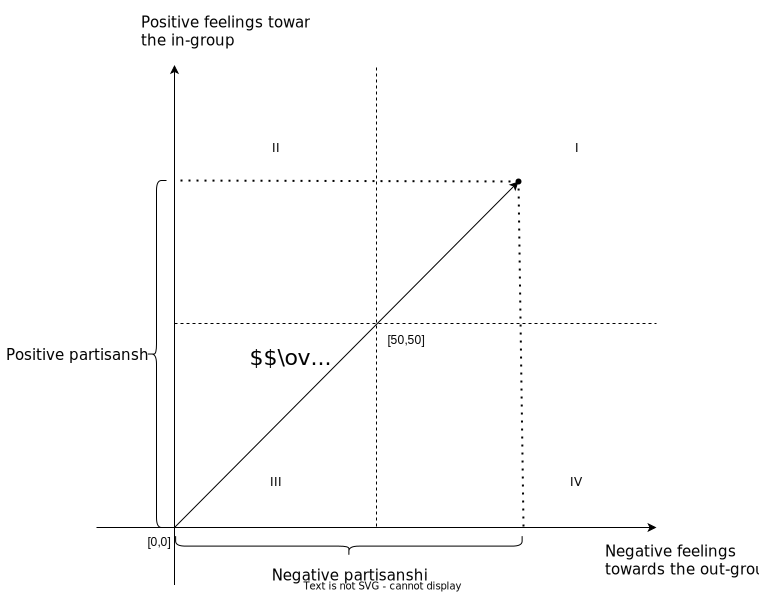
\includegraphics[width=\textwidth]{Figures/API-theory.pdf}
	\label{fig:types_and_levels_of_AP}
\end{figure}


To better see my characterization of \textbf{amount} and \textbf{types} of affective polarization, see Figure \ref{fig:types_and_levels_of_AP}. I plot two perpendicular axes representing the feelings thermometer commonly used in surveys, in this case ranging from -50 to 50 in order to ease the interpretation by letting [0,0] in the center of the axes. The two axes define a two-dimensional space in which the horizontal dimension represents the feelings someone has towards his/her out-group and the vertical dimension represents the feelings someone has towards his/her in-group. The extremes represent very good (50) or very bad (-50) feelings towards each group. In this plane, a point represents the combination of these two feelings. The total amount of polarization for an individual can be computed as the absolute value of the difference between these two thermometer ratings. Additionally, in line with both \citet*{Wagner2021} and \citet*{Reiljan2020}, in order to be precise, we should account for party size. Consider party size as a factor that scale the contribution each party makes to both the in-group and the out-group. Thus, to like or to dislike bigger parties has a larger impact on the final Affective Polarization Index (API) score. Hence, if we use the standardized vote share to weight parties, API is, more formally:

$$
	\text{Affective Polarization Index}_i = \lvert a_i - b_i \rvert
$$

where $a$ and $b$ are the weighted average of the distances measured on the vertical and horizontal axis respectively from the [0,0], that is:

$$
	a_i, b_i = \sqrt{\sum^p_{p=1}{\nu_p*\text{like}_{ip}}}
$$

where ``like" is the already mentioned feelings thermometer score, $p$ represents the parties in each of the two groups and $\nu_p$ is the normalized (relative to the total of relevant parties included)\footnote{In the operationalizaition section I discuss this more in depth, however, to better understand what I mean notice that since I only include the main 5 parties in the Spanish system, the total vote share does not add up to 100\%. Hence, the vote share is standardized to range from 0 to 1 by simply dividing each party vote share by the total share these 5 parties represent.} vote share of party $p$.

Thus, the amount of affective polarization grows from the first and third quadrants bisector outwards. The further the point is from the function $y=x$ the more polarized someone is. Hence, people laying at a similar distance from $y=x$ have a similar amount of affective polarization, however, this amount can be caused by several combinations of the two components, that is, by different levels of positive and negative feelings. This proposal is assuming two things: first, the in-group and the out-group must be defined beforehand and explicitly. In general, they should coincide with incumbent vs opposition to study an accountability mechanism, but in the specific case of Spain it also coincides with the two ideological blocks suggested by \citet*{Orriols2020}; and second: the score summarizing positive and negative feelings towards each group must be an average of the scores for each of the parties in those groups. This average might or not be weighted accounting for party size. To see a discussion about the consequences of weighting parties when computing affective polarization indexes, see \citet*{Wagner2021}.

Although it is reasonable to expect that --in general terms-- partisans will be more inelastic than non-partisan voters, the interesting part of the argument to be tested is the extent to which affective polarization moderates the level of economic voting of those who identify with the incumbent or those who doesn't. Hence, in both groups, those who are incumbent voters and those who aren't, it is expected to find what I call \textit{supporters}, people with average to high levels of elasticity; what I call \textit{regular partisans} with average levels of (lack of) elasticity and \textit{fans}, with very low levels of elasticity. These three groups are intended to simplify the interpretation and their names are contingent. What is important is to have a group with average levels of polarization, a group below it and a group above it. Based on these three groups, in theory, we should see a distribution of affects and hence a distribution of the API as showed in Figure \ref{fig:empirical_expectations}.

\begin{figure}[H]
	\centering
	\includegraphics[width=\textwidth]{Figures/Expected empirics.pdf}
	\caption{Expected distribution of Affective Polarization components}
	\label{fig:empirical_expectations}
\end{figure}



Moreover, although the theory suggests a plane divided into four quadrants, only three of those are logical. Most of the people should lay on the second quadrant where positive feelings towards the in-group are larger than feelings towards the out-group. Some people could lay on the first quadrant, where feelings towards both the in-group and the out-group are larger than 50; these people are supposed to have a general positive image of the political parties. Conversely, those laying on the third quadrant have negative feelings towards both groups, hence, they are characterized by a negative image towards the politicians as a whole. Finally, people laying in the fourth quadrant should be outliers and rare cases since these people would have better feelings towards their out-group than towards their in-group, which makes no sense according to the theory advanced here. To summarize, elasticity is a function of positive and negative partisanship. One of the goals of the present study is to disentangle these effects in order to better understand affective polarization when it is separated in its two constituent components.

\newpage

\section{Hypotheses}

As noted in the previous section, I will clearly split the sample into two groups to run the analyses. On the one hand, people whose in-group include the incumbent. This is to say that either they identify with one of the parties in the government or they declare that they would ever vote for one of them\footnote{This is a consequence of the limitations of the dataset. Although more information is provided in the research design section, note that the dataset is divided in waves. Only one of the four waves includes a question explicitly asking for party identification.}. On the other hand, people that declare to be an opposition supporter. The latter potentially would never vote for the incumbent, nonetheless, the same analysis is also run restricting the sample to them because the theory is general enough as to ask for the effects of affective polarization on economic voting for everyone voting.

Within these groups, I define three more groups to categorize somehow the level of polarization. According to the theory proposed, people can be characterized either as a \textit{supporter}, a \textit{regular partisan} or a \textit{fan} according to its level of affective polarization and, subsequently, elasticity. Hence, for the sake of simplicity, I will now define the groups of people involved and the theoretical expectations that would ultimately yield the different empirical hypotheses to be tested.

First, people is identified either as someone willing to vote for the incumbent (e.g. potential incumbent voters) or someone willing to vote for any opposition party (e.g. opposition voters). This means that people reporting to be not sure about which party they would vote for in a hypothetical election, or people reporting that they would not vote are excluded from the analysis. Second, within each group, we can further distinguish three groups of voters according to its level of elasticity. On the extremes I identify: on the one hand people with low to average levels of affective polarization (supporters) and, on the other hand, people with average to high levels of affective polarization (fans). In the middle, we identify those with average levels of affective polarization (regular partisans).

As noted before, it is mandatory to define the in-group and the out-group beforehand so, in order to simplify things, I will use in a first approximation the incumbent or governing parties as the in-group and the rest of the main parties as the out-group. Probably, the most accurate split would be between incumbent and opposition considering ideological blocks, but nevertheless, in Spain these two things coincide. PSOE and Podemos (the left-wing ideological block) are the governing parties during the period analyzed and the rest of the main parties included in the analysis represent the right-wing ideological block.

The theory advanced here tells us that among those who rate the state of the economy as worse when asked, polarized incumbent's potential voters should be more willing to vote for it. Conversely, polarized opposition's voters should avoid reward the incumbent if economy goes good. That is to say that economic voting work worse the more polarized people are. Therefore the main general hypothesis can be written as follows:

\textit{H1: The more affectively polarized an individual is, the less important his/her economic assessment is to understand his/her likelihood of voting for the incumbent in a future election.}

In order to be more precise exploring the empirical implications of the theory, I turn to formulate the specific hypotheses for each group of voters.

\subsection{Incumbent's potential voters}

According to the argument proposed in section \ref{section:theory} I expect incumbent's supporters likelihood of voting for the incumbent higher the more polarized they are. Therefore:

\textit{H2: Incumbent's \textbf{fans} are \textbf{more} willing to vote for the incumbent than regular partisans and supporters respectively.}

And related to H1 but applied for incumbent's potential voters, we can formulate the following hypotheses according to the proposed categorization of the elasticity an individual has because the three groups are supposed to be ranked in a certain order. Therefore, I can propose the following hypotheses:

\textit{H2a: Among those who assess the economy as \textbf{worse} than in the past and are identified as incumbent's potential voters, \textbf{fans} are \textbf{more} willing to vote for the incumbent than regular partisans and supporters respectively.}

Since the affective polarization measure is expected to be lineal:

\textit{H2b: Among those who assess the economy as \textbf{worse} than in the past and are identified as incumbent's potential voters, \textbf{regular partisans} are \textbf{more} willing to vote for the incumbent than supporters.}

\subsection{Opposition's potential voters}

Regarding opposition voters, they are supposed not to be willing to vote for the incumbent in a future election by definition. However, it is reasonable to think that some of the opposition voters would be able to reward the incumbent if the economy goes better. In fact, otherwise the electoral results would never change. Thus, a general hypothesis regarding the level of elasticity can be formulated:

\textit{H3: Opposition \textbf{fans} are \textbf{less} willing to vote for the incumbent than regular partisans and supporters respectively.}

Hence, among those who assess the economy as better, I expect those more polarized (fans) to be less willing to vote for the incumbent than supporters and partisans respectively. Therefore:

\textit{H4a: Among those who assess the economy as \textbf{better} than in the past, and are identified as opposition voters, \textbf{fans} are \textbf{less} willing to vote for the incumbent than regular partisans and supporters respectively.}

Once again, since the affective polarization measure is expected to be lineal:

\textit{H4b: Among those who assess the economy as \textbf{better} than in the past, and are identified as opposition voters, \textbf{regular partisans} are \textbf{less} willing to vote for the incumbent than supporters.}

Even when these groups of hypotheses are able to account for all possible combinations between level of affective polarization and strength of economic voting, we don't know yet if the relationship is driven by negative or positive partisanship. In fact, because of how I have phrased them, I am assuming that somewhat it is positive partisanship what drives the results. This is because everything here gravitates around the incumbent: if you are expected to support the incumbent, in case of polarization it should be due to positive partisanship, that is, because the positive feelings towards the in-group make you exonerate the incumbent. Or in other words, the more polarized you are, the closer you are to the incumbent. This would yield the following hypothesis:

\textit{H5a: For incumbent's potential voters, the better the feelings towards the in-group, the higher their likelihood of voting for the incumbent.}

However, as discussed in the previous section, affective polarization is made up of two components (positive and negative partisanship) and so that could not necessarily be the case. It is reasonable to see people that, contrary to H5a, hate the out-group very much. Since these two hypotheses are not exclusionary \textit{stricto sensu} because both things can happen at the same time, the following hypothesis is also subject to be empirically tested:

\textit{H5b: For incumbent's potential voters, the worse the feelings towards the out-group, the higher their likelihood of voting for the incumbent}




\section{Research design}

\label{section:research_design}

Since my hypotheses refer to individuals I use a micro level database to empirically test them. Data comes from the E-DEM dataset, a new micro-level online panel survey of the Spanish voting age population with more than 8.100 interviews collected \citep{Torcal2020}. Although I could have followed a more comparative approach using, for instance, CSES data, I still think that Spain is an interesting case where testing my hypotheses. Moreover, given my theoretical expectations, a comparative approach would imply a huge effort categorizing first which parties conform the incumbent and which ones the opposition in each country, along with accounting for the voting patterns in all of them. This is, of course, an interesting design for future research but, unfortunately, it lays out of the scope of a Master Thesis. On the contrary, using this dataset I can leverage my knowledge of the Spanish system and I can track individuals' opinions and their assessment of the economy during a crucial period in Spanish recent politics.

This dataset contains four waves spanning a period between October 2018 and May 2019. Although short, during that period of time most of the key political events affecting Spanish politics after 15M happened: for instance, local, regional, national and European elections took place within this period, but also the conviction of Catalan secessionist leaders. And, more importantly, it also covers the six-month period of surge of Spain's new radical right party, Vox \citep{Torcal2020}. This last event is expected to be very related to the increase of affective polarization levels in Spain (either as a cause or a consequence). An important caveat to make is that unfortunately, although data is panel I cannot leverage this feature since most of the questions about future elections are only asked in certain waves. Hence, I use the data as a pool of more than one period but there is not an actual temporal dimension. Also because of that and to avoid unnecessary complexity, I drop observations from wave 1 in which the incumbent was the Partido Popular (PP). This would yield approximately 7500 valid observations. However, since I only have information about vote intention for the last two waves, observations drop to a maximum of 5000, a still good number to work with.

This dataset also contains both variables capturing individuals assessment of the economy, and a lot of sociodemographic variables useful to control for. There are questions about leaders' assessment and party identification and even more importantly, although the usual feelings thermometer question is also present in the dataset and will be used as a benchmark, there are several questions similar to this included like ``feelings towards people from certain regions", ``feelings towards voters of certain parties", and ``feelings towards party leaders". Thus, I can use measures of affective polarization different from the usual thermometer scale. In fact, I think that, especially ``feelings towards voters of different parties", would be an even more accurate measure of affective polarization as described in section \ref{affective polarization} since instead of asking about parties, respondents are asked about their feelings towards voters. The scale is slightly different to the usual one (0-10), it ranges from 0 to 100 with jumps of 15 points. Nonetheless, I can still build the API based on the two components mentioned in section \ref{section:theory} and, for reproducibility purposes, this measure could still fit \cite{Wagner2021}'s formula. Let me now define all the intervening variables.

\subsection{Dependent Variable}

My dependent variable is simply a dummy variable taking on value 1 if someone reports to be willing to vote for the incumbent in a hypothetical future (national) election. The non-trivial part, however, is to define the incumbent given that during the period considered the first coalition government at the national level in Spanish electoral history (since the Spanish Second Republic) was formed. There are different possibilities\footnote{See the appendix to see an analysis of them} but my preferred one (and closest to reality) is the one in which both PSOE (in wave 3) and Podemos (along with PSOE in wave 4) are considered to be the incumbent. It is important to note that this variable is constructed in a rather convoluted way because of data constraints. Ideally, I would use either actual vote recall or vote intention in a certain election. However, since the time span of the survey only covers April 28th national elections, I have combined two different variables to construct my dependent variable. As explained above, I can only use third and fourth waves pooled together but only in wave 3 there is the proper question about vote intention. Hence, for wave 4 I use a question about the probability of ``ever voting for'' different parties as a proxy. In that case, those reporting a probability equal or grater than 5 of voting for either PSOE or Unidas Podemos (in the respective waves) are considered a 1, the rest are considered a zero.

\subsection{Explanatory varaibles}

\subsubsection{Affective Polarization Index}

The usual way of measuring affective polarization is the one used by \cite{Gidron2018}. They use survey data from a module of the CSES asking respondents to rate political parties in the classical 0-10 thermometer scale (that is, how much they like or dislike a certain party). After that, they basically inverse the scale so that 10 denotes the most negative party evaluation and 0 the most positive. However, instead of calculating an average level of affective polarization, I need to compute the individual amount of polarization. In order to be able to benchmark my own theoretical proposal (see section \ref{theoretical-proposal}), I will run the main analyses with my own API and I will add a section in the \hyperref[appendix]{Appendix} using \citet{Wagner2021}'s formula. I believe this is a good empirical exercise since \citeposs{Wagner2021} index is the best we have to date to measure affective polarization at the individual level in multiparty systems.

As defined in \ref{theoretical-proposal}, API is the absolute value of the difference between the weighted average level of affect towards someone's in-group and the weighted average level of affect towards someone's out-group. These two components, in order to yield observations in a space with [0,0] as the reference (or neutral) point, must be slightly modified:

$$
	\text{Feelings towards the in-group/out-group} = \sqrt{\sum^p_{p=1}\nu_p(\text{like}_{ip}-50)}
$$

the group of parties $p$ is defined as follows: the in-group is conformed by PSOE and Unidas Podemos for incumbent's potential voters, whereas the out-group is conformed by PP, Ciudadanos\footnote{Ciudadanos is included in this group because they rejected the possibility of forming government with PSOE in April 2019 election. Moreover, as suggested in \citet*{Orriols2020}, left-wing voters' rejection of C's and Vox peaked during this period} and Vox for these voters. For opposition's voters, these groups are just the opposite. $\nu_p$ is the relative weight of each party according to its vote share normalized from 0 to 1. Given that only these 5 parties are included in the analyses, the total vote share does not add up to 100\%. To overcome this, each party vote share is divided by the total share represented by those 5 parties by wave.

A first benchmark to see to what extent API is compatible with \citeposs{Wagner2021} formula is to see the correlation between these two variables. Correlation coefficient is 0.9123 ($p<0.000$)(see Figure \ref{fig:corr-api-wap} in the \hyperref[appendix]{Appendix}).

As suggested in section \ref{section:theory} elasticity of voters is defined by their level of affective polarization. An easy and \textit{a priori} objective way to define the typology of voters according to its level of elasticity is to cut the API in three slices according to the standard deviation. Hence, \textit{\textbf{supporters}} would be those whose affective polarization level is below one standard deviation, \textit{\textbf{partisans}} would be defined as those between minus one and plus one standard deviations and \textit{\textbf{fans}} are defined as those above one standard deviation. That yields the next distribution of voters:

\begin{table}[H]
	\centering
	\caption{Groups of incumbent's potential voters according to its level of Affective Polarization}
	\label{tab:groups}
	\begin{tabular}{@{}lcc@{}}
		\toprule
		           & Observations & Percentage \\ \midrule
		Supporters & 196          & 18.88      \\
		Partisans  & 669          & 64.45      \\
		Fans       & 173          & 16.67      \\
		Total      & 1,038        & 100.00     \\ \bottomrule
	\end{tabular}
\end{table}

And if we now look at Figure \ref{fig:pos_neg_incumbent} we see the distribution of the two components (positive and negative partisanship) for potential incumbent's voters.

\begin{figure}[H]
	\centering
	\includegraphics[scale=0.3]{Figures/pos_neg_groups.png}
	\caption{Positive and Negative Partisanship for potential incumbent's voters}
	\label{fig:pos_neg_incumbent}
\end{figure}

We can see that, as expected, most of the potential incumbent's voters, lay on the second quadrant and, more importantly, polarization grows from $y=x$ outwards. We also see some extreme cases in the first quadrant that are either PSOE or Unidas Podemos voters that have positive feelings towards part of the out-group, recall that Ciudadanos is in the out-group for these voters. For a complete picture of the distribution of the two components of affective polarization by party, refer to Figure \ref{fig:pos-neg-parties}.

\subsubsection{Economic assessment}

As a measure of national economy assessment made by respondents, E-DEM dataset includes the arguably most straightforward and common question about economic assessment. Respondents are not asked to give a very precise assessment of the economic situation, they are just asked if they think economy is either better or worse than in the last 12 months.
The variable as it appears in the dataset takes on values 1 (``A lot worse'') to 5 ``A lot better''. I recode this variable to have three categories: ``worse", ``no difference'' and ``better''. The goal is to ease the interpretation of the results focusing on the change from a negative assessment to a positive one. Nonetheless, I keep the neutral category because it is the most populous one (almost 42\% of observations).


\begin{table}[H]
	\centering
	\caption{Assessment of the Spanish economy}
	\label{tab:economic assessment}
	\begin{tabular}{@{}lcc@{}}
		\toprule
		                & Observations & Percentage \\ \midrule
		A lot worse     & 654          & 11.68      \\
		A little worse  & 1,271        & 22.70      \\
		No difference   & 2,326        & 41.54      \\
		A little better & 1,314        & 23.47      \\
		A lot better    & 34           & 0.61       \\
		Total           & 5,599        & 100.00     \\ \bottomrule
	\end{tabular}
\end{table}

\subsubsection{Control variables}
My control variables are common sociodemographic controls that might influence the likelihood of voting for the incumbent. They are the region (autonomous community) the individual comes from, sex, age, size of the habitat individual lives, martial status, educational level attained, occupation, income and religious beliefs.


\subsection{Models}

I use logit models to estimate the likelihood of voting for the incumbent. The general equation is as follows:

\begin{equation}
	\label{model}
	y_i = \beta_1 x_{1i} + \beta_2 x_{2i} + \beta_3 Z_i  + \eta_i  + \epsilon_i
\end{equation}

where $y_i$ is a dummy variable taking on value 1 if the respondent will vote for the incumbent in the following election and 0 otherwise\footnote{For respondents in wave 4, since there is no question asking about a hypothetical future election, a 1 represents people with a score of more than 5 in the question about the probability of ever voting for either PSOE or Unidas Podemos (Podemos+IU)}, $\beta_1$ is the expected effect of economic voting (i.e. the likelihood of voting for the incumbent according to economic assessment) alone, $\beta_2$ is the effect of affective polarization\footnote{In some specifications, this variable is a continuous measure, in others it is a dichotomous one, splitting the sample between those above and those below the average level of affective polarization} on the probability of voting for the incumbent and, the outcome of interest, $\beta_3$ is the interaction between both $x_1$ and $x_2$. Thus, $\beta_3$ captures the effect of economic voting according to the level of affective polarization of the individual. Finally, $\eta_i$ is a vector of sociodemographic control variables, and $\epsilon$ is the error term.

The same model is estimated when focusing on the components of the API. in that case, $\beta_1$ would still represent the effect of economic voting on the likelihood of voting for the incumbent, whereas $\beta_2$ would represent te effect of either positive or negative partisanship. Finally, $\beta_3$ is again the interactive effect between the component and the economic voting variable.

\section{Affective Polarization in Spain (descriptive results)}

Once I have presented my research design it is worthwhile to explore the data to have an image of Affective Polarization in Spain. I first include two general pictures of the API distribution. One distinguishing between government and opposition partisans (Figure \ref{fig:AP_partisan}) and a second one distinguishing by party identity (Figure \ref{fig:AP_party_id}).

We can see that the distribution of the API does not follow a normal distribution for neither the incumbent voters and opposition voters. Importantly, there are a lot of zeros for the case of opposition voters what is suggesting a smaller level of affective polarization on average. In fact, it is interesting to see that incumbent voters (Mean = 9.605; SE = 0.168) are significantly more polarized on average than opposition ones (Mean = 7.780; SE = 0.184) (Diff = 1.83; SE = 0.249). This lack of normality can be a concern for the results when trying to estimate the equations, nonetheless, it is important to note that Wagner's WAP distribution is quite similar (see Figure \ref{fig:WAP_oppo_incumb} in the \hyperref[appendix]{Appendix}).

\begin{figure}[H]
	\centering
	\caption{\label{fig:AP_partisan} Incumbent vs Opposition API distributions}
	\includegraphics[scale=0.25]{Figures/AP_index_by_partisanship.png}
\end{figure}

If we take a look now at the distribution of polarization by party (Figure \ref{fig:AP_party_id}), we also observe some interesting patterns. First, distributions look more different compared to each other than opposition vs incumbent voters. Nevertheless, we can see that parties' affective polarization means' ranking is somehow related to the position they hold in the ideological scale (the closer to the center, the less polarized they seem). Vox and Unidas Podemos are the most polarized on average, PP and PSOE are less so, and Ciudadanos voters are the ones with the smallest score\footnote{All the descriptive statistics can be found tabulated in the \hyperref[appendix]{Appendix}}. We find that Unidas Podemos voters are significantly more polarized than PP (Diff=1.802, $p<0.000$), Ciudadanos (Diff=5.533, $p<0.000$) and PSOE (Diff=1.674, $p<0.000$) voters; PSOE voters are significantly more polarized than Ciudadanos (Diff=3.858, $p<0.000$), finally, Ciudadanos voters are significantly less polarized than VOX (Diff=-4.966, $p<0.000$) and PP (Diff=-3.731, $p<0.000$) voters respectively. The remaining differences are not statistically different from zero.

These patterns are suggesting that affective polarization at the individual level is quite close to ideological polarization. However, we cannot say anythin conclusive only with this descriptive data, it is interesting to find parties ranked as they are in ideological terms. That makes sense since parties closer to the extremes (ideologically) are --by definition-- farther from the outgroup. Hence, negative feelings could play a role. On the contrary, parties closer to the center, specially Ciudadanos, may have voters close enough to both the in-group and the out-group (recall that these groups are defined beforehand which is a logical limitation to this analysis). Thus, Ciudadanos voters positive and negative feelings might counteract to a larger extent. Moreover, it is very clear that Ciudadanos, PP and PSOE respectively, are the parties with more people with a level of zero affective polarization. To see a more specific picture of positive and negative partisanship, see Figure \ref{fig:pos-neg-parties}.


\begin{figure}[H]
	\centering
	\includegraphics[width=\textwidth]{Figures/AP_index_by_party_id.png}
	\caption{\label{fig:AP_party_id} Affective Polarization Index by party identification}
\end{figure}

It can be seen at first sight that parties on the right (Ciudadanos, PP and Vox) tend to have a smaller in-group feeling, thus, leveraging the fact that parties are an ideological mirror in Spain, that is, that placing Ciudadanos in the middle, we have two moderate and two extrem parties to the right and to the left, we can infer that PSOE voters affective polarization level is driven by positive partisanship to a large extent, whereas PP affective polarization level is driven to a larger extent by negative partisnahip. Something similar can be said about Unidas Podemos and Vox. Overall, left-wing parties seem to be closer to their in-group whereas right-wing parties tend to be farther from their out-group. In fact, if we look for the difference in a more precise way, positive partisanship is significantly larger on average for incumbent parties (left-wing parties) at the 95\% level (Diff=2.955, $p<0.000$). And also, although differences are smaller, negative partisanship is larger (and negative) on average for opposition parties (Diff=0.683, $p<0.001$).


\begin{figure}[H]
	\centering
	\includegraphics[width=\textwidth]{Figures/pos_neg_parties.png}
	\caption{Positive and Negative partisanship by party id}
	\label{fig:pos-neg-parties}
\end{figure}


Now that we have seen the distribution of the API and its components for each of the main parties, it is interesting to say something about feelings inter parties. In Figure \ref{fig:feelings} we can see the distance in feelings towards \textbf{voters} of each party for those whose level of affective polarization is above and below the average. This is an important measure because reveals the extent to which positive and negative partisanship is present in the Spanish system. The horizontal axis plots the level of warmness that an individual has regarding voters of every one of the five biggest parties. It ranges from 0 being feeling very cold to 100 being feeling very close or warm. In the vertical axis I separate the results for each party to explore the plausible heterogeneity. The parties are ordered according to their position in the ideological scale (left to right is top to bottom) in order to ease the interpretation of the results. The results are very robust.


First of all, for every party, voters more affectively polarized (red) are closer to their party, that is, positive partisanship towards own's party plays a crucial role. This is specially the case for Vox, the party with the largest score\footnote{To see these distances plotted as punctual estimations, see Figure \ref{fig:dot-distances} in the \hyperref[appendix]{Appendex}}. Also and once again, we can see that the in-group and the out-group as previously defined are playing the expected role. For every party, more polarized voters belonging to the in-group tend to feel closer to that party, whereas more polarized voters of the out-group tend to feel farther. Finally, we can also observe the importance of less polarized voters (i.e. moderate voters) within parties. For example, less polarized voters of Ciudadanos and PP are on average close to 50 in the feelings termomether with respect to PSOE, whereas more polarized ones, are clearly cooler.

\begin{figure}[H]
	\centering
	\includegraphics[width=\textwidth]{Figures/combinedfeelingsAP.png}
	\caption{\label{fig:feelings} Feelings towards party voters and affective polarization}
\end{figure}

The reason behind plotting parties ordered by ideology in the vertical axis is to better see that except for Ciudadanos who is put at the end of the panel on purpose, we see a mirror image on the pattern. In line with \citep*{Orriols2020}, there is a clear pattern regarding the out-group formation that basically has to do with two ideological blocs. If we look at Figure \ref{fig:feelings} by rows, we see that left parties' voters display feelings that are a mirror image of those of the rightwing voters. Moreover, the spread of those feelings, in line with \citep*{Wagner2021} is grater as the parties move apart ideologically, that is, feelings towards both the in-group and the  out-group are more extreme for UP and VOX voters than they are for PSOE and PP respectively. Interestingly if we focus now on Ciudadanos, we see that for leftist voters (PSOE and UP), it is clearly considered a party belongin to the out-group. Especially for those more affectively polarized. Conversely, PP and VOX voters have positive feelings towards Ciudadanos, espcially the more polarized they are. Nonetheless, PP voters seem to like Ciudadanos voters regardless of the level of polarization. This is also true for Ciudadanos voters feelings towards PP, meaning that these parties' voters are both in the same group. Vox voters, on the contrary, only display positive feelings towards these two parties the more polarized they are. For voters less polarized than the average, feelings are quite neutral what may explain, once again, the small amount of positive partisanship for this group of parties.

\newpage

\section{Results}

Now we turn to the main results of the paper. In this section I summarize and discuss the empirical evidence for or against my main hypotheses. I expect the relationship between affective polarization and economic voting to be inverse. In other words, I expect those less polarized to display a ``normal'' relationship between economic assessment and likelihood of voting for the incumbent. This relationship become ``abnormal'' the more polarized they are. In order to see this empirically, I compare the groups distinguishing between those who rate the economy as worse than in the past and those who rate the economy as better.

In order to be consistent with how I have presented my hypotheses, I will divde this section into two subsections, one for the analysis of incumbent's potential voters and another one for oppostion's voters.

\subsection{Incumbent's potential voters}

\begin{table}[H]
	\label{main_results}
	\centering
	\caption{\label{tab:incumbent} Effects of affective polarization on economic voting (incumbent's poential voters)}
	{
\def\sym#1{\ifmmode^{#1}\else\(^{#1}\)\fi}
\begin{tabular}{l*{5}{c}}
\toprule
                &\multicolumn{5}{c}{Likelihood of voting for the incumbent}                                    \\\cmidrule(lr){2-6}
                &\multicolumn{1}{c}{(1)}         &\multicolumn{1}{c}{(2)}         &\multicolumn{1}{c}{(3)}         &\multicolumn{1}{c}{(4)}         &\multicolumn{1}{c}{(5)}         \\
\midrule
Economic assessment (ref.: Better)&                  &                  &                  &                  &                  \\
Worse           &    0.767         &    0.880         &    1.223         &    0.869         &    1.178         \\
                &  (-1.15)         &  (-0.54)         &   (0.48)         &  (-0.60)         &   (0.35)         \\
Affective Polarization Index&                  &    1.053\sym{***}&    1.081\sym{***}&                  &                  \\
                &                  &   (3.66)         &   (3.49)         &                  &                  \\
Worse $\times$ Affective Polarization Index&                  &                  &    0.965         &                  &                  \\
                &                  &                  &  (-0.84)         &                  &                  \\
Wagner's (2021) WAP index&                  &                  &                  &    1.020\sym{***}&    1.033\sym{***}\\
                &                  &                  &                  &   (3.56)         &   (3.59)         \\
Worse $\times$ Wagner's (2021) WAP index&                  &                  &                  &                  &    0.989         \\
                &                  &                  &                  &                  &  (-0.63)         \\
\midrule
Pseudo \(R^{2}\)&    0.014         &    0.026         &    0.028         &    0.025         &    0.028         \\
Observations    &     1037         &     1036         &     1036         &     1026         &     1026         \\
\bottomrule
\multicolumn{6}{l}{\footnotesize Exponentiated coefficients; \textit{t} statistics in parentheses}\\
\multicolumn{6}{l}{\footnotesize NOTE: All the specifications include the following control variables: sex, age, place of residence, marital status,}\\
\multicolumn{6}{l}{\footnotesize education, occupation, income and religious beliefs. They are excluded from the table for clarity reasons.}\\
\multicolumn{6}{l}{\footnotesize \sym{*} \(p<0.05\), \sym{**} \(p<0.01\), \sym{***} \(p<0.001\)}\\
\end{tabular}
}


\end{table}

Looking at Table \ref{tab:incumbent} we can see that contrary to what could be expected, the economic assessment variable (i.e. economic voting) does not work in any specification. Economic voting was expected to work better among opposition supporters, however, for incumbent's potential voters, the fact that a change in the assessment of the economy does not produce any effect on the likelihood of voting for the incumbent, breaks the model and makes very difficult to interpret the rest of the coefficients. In fact, $\beta_3$, that is, the effect of economic voting conditional on the level of polarization is not significant either. Nevertheless, in most of the specifications (1, 2, 4) these coefficients have the predicted sign.

All we can say about this table is that the API has a positive and significant effect on the likelihood of voting for the incumbent. Hence, this is evidence in favor of \textit{H2}. This could be suggesting that the API is a good predictor of the likelihood voting for the incumbent but there is no effect of affective polarization on accountability. In order to see this more visually, in Figure \ref{fig:margins} I plot margins at different levels of elasticity and economic assessment.

\begin{figure}[H]
	\centering
	\includegraphics[width=0.7\textwidth]{Figures/margins.png}
	\caption{\label{fig:margins}Margins of economic voting and elasticity }
\end{figure}


\begin{table}[H]
	\label{inc-pos-neg}
	\centering
	\caption{\label{tab:incumbent-pos-neg} Effects of affective polarization components on economic voting}
	{
\def\sym#1{\ifmmode^{#1}\else\(^{#1}\)\fi}
\begin{tabular}{l*{3}{c}}
\toprule
                &\multicolumn{3}{c}{Likelihood of voting for the incumbent}\\\cmidrule(lr){2-4}
                &\multicolumn{1}{c}{(1)}         &\multicolumn{1}{c}{(2)}         &\multicolumn{1}{c}{(3)}         \\
\midrule
Economic assessment (ref.: Worse)&                  &                  &                  \\
Better          &    1.125         &    1.037         &    0.947         \\
                &   (0.50)         &   (0.11)         &  (-0.17)         \\
Feelings towards the in-group&    1.088\sym{***}&    1.088         &    1.089\sym{***}\\
                &   (4.74)         &   (1.83)         &   (4.78)         \\
Feelings towards the out-group&    0.998         &    0.998         &    1.002         \\
                &  (-0.09)         &  (-0.10)         &   (0.04)         \\
Better $\times$ Feelings towards the in-group&                  &    1.014         &                  \\
                &                  &   (0.26)         &                  \\
Better $\times$ Feelings towards the out-group&                  &                  &    0.960         \\
                &                  &                  &  (-0.67)         \\
\midrule
Pseudo \(R^{2}\)&    0.034         &    0.034         &    0.036         \\
Observations    &     1035         &     1035         &     1035         \\
\bottomrule
\multicolumn{4}{l}{\footnotesize Exponentiated coefficients; \textit{t} statistics in parentheses}\\
\multicolumn{4}{l}{\footnotesize NOTE: All the specifications include the following control variables: sex, age, place of residence, marital status,}\\
\multicolumn{4}{l}{\footnotesize education, occupation, income and religious beliefs. They are excluded from the table for clarity reasons.}\\
\multicolumn{4}{l}{\footnotesize \sym{*} \(p<0.05\), \sym{**} \(p<0.01\), \sym{***} \(p<0.001\)}\\
\end{tabular}
}


\end{table}

Something similar is in Table \ref{tab:incumbent-pos-neg}. None of the economic voting variables have an effect statistically different from zero on the likelihood of voting for the incumbent. Again, most of them have the expected sign, but no significance. However, it seems that feelings towards the in-group has a positive and significant effect on the likelihood of voting for the incumbent, what is evidence in favor of H2a and agiainst H2b. This suggests that for incumbent's potential voters, is positive partisanship what drives affective polarization.

\begin{figure}[H]
	\centering
	\includegraphics[width=\textwidth]{Figures/pos-neg.png}
	\caption{\label{fig:pos-neg-inc-margins} Economic voting and positive and negative partisanship for incumbent's potential voters}
\end{figure}


\subsection{Opposition's potential voters}

\begin{table}[H]
	\centering
	\caption{\label{tab:opposition} Effects of affective polarization on economic voting (opposition's poential voters)}
	{
\def\sym#1{\ifmmode^{#1}\else\(^{#1}\)\fi}
\begin{tabular}{l*{5}{c}}
\toprule
                &\multicolumn{5}{c}{Likelihood of voting for the incumbent}                                    \\\cmidrule(lr){2-6}
                &\multicolumn{1}{c}{(1)}         &\multicolumn{1}{c}{(2)}         &\multicolumn{1}{c}{(3)}         &\multicolumn{1}{c}{(4)}         &\multicolumn{1}{c}{(5)}         \\
\midrule
Economic assessment (ref.: Worse)&                  &                  &                  &                  &                  \\
Better          &    3.270\sym{**} &    3.025\sym{**} &    2.130         &    2.853\sym{*}  &    2.649         \\
                &   (2.93)         &   (2.67)         &   (1.27)         &   (2.47)         &   (1.27)         \\
Affective Polarization Index&                  &    0.819\sym{***}&    0.800\sym{***}&                  &                  \\
                &                  &  (-5.01)         &  (-3.50)         &                  &                  \\
Better $\times$ Affective Polarization Index&                  &                  &    1.089         &                  &                  \\
                &                  &                  &   (0.83)         &                  &                  \\
Wagner's (2021) WAP index&                  &                  &                  &    0.972\sym{**} &    0.974         \\
                &                  &                  &                  &  (-2.61)         &  (-1.56)         \\
Better $\times$ Wagner's (2021) WAP index&                  &                  &                  &                  &    1.004         \\
                &                  &                  &                  &                  &   (0.12)         \\
\midrule
Pseudo \(R^{2}\)&    0.096         &    0.175         &    0.176         &    0.106         &    0.107         \\
Observations    &      981         &      980         &      980         &      967         &      967         \\
\bottomrule
\multicolumn{6}{l}{\footnotesize Exponentiated coefficients; \textit{t} statistics in parentheses}\\
\multicolumn{6}{l}{\footnotesize NOTE: All the specifications include the following control variables: sex, age, place of residence, marital status,}\\
\multicolumn{6}{l}{\footnotesize education, occupation, income and religious beliefs. They are excluded from the table for clarity reasons.}\\
\multicolumn{6}{l}{\footnotesize \sym{*} \(p<0.05\), \sym{**} \(p<0.01\), \sym{***} \(p<0.001\)}\\
\end{tabular}
}


\end{table}

In table \ref{tab:opposition} we see results for opposition's supporters. As discussed in section \ref{section:theory}, economic voting's effect here is much more powerful. In almost every specification, the effect is positive and statistically significant. Moreover, the effect of the API is, as expected, opposite to incumbent's potential voters. Here, the effect is negative, meaning that the more polarized they are, opposition's potential voters are less willing to vote for the incumbent, which is evidence in favor of H3. Unfortunately, regarding effects of affective polarization on economic voting, once again, all the coefficients have the sign predicted by the theory but are not distinguishable from zero.

Finally, in table \ref{tab:oppo-pos-neg}, we find that economic voting also works as expected, the better voters rate the economy, the more willing they are to vote for the incumbent. Regarding feelings towards the in-group and the out-group, here we find, interestingly, that both have a significant effect. In fact, both have the predicted sign. The interpretation of these coefficients though is not trivial. Recall that these are opposition's potential voters, hence, here the in-group is the opposition whereas the out-group is the incumbent. Therefore, we find that the closer to the in-group an opposition's potential supporter  is the less willing he/she is to vote for the incumbent. But it is also true that the more they like their out-group, that is, the incumbent, the more willing they are to vote for it. This yields evidence in favor of H5a and H5b.

\begin{table}[H]
	\centering
	\caption{\label{tab:opposition-pos-neg} Effects of affective polarization components on economic voting}
	\label{tab:oppo-pos-neg}
	{
\def\sym#1{\ifmmode^{#1}\else\(^{#1}\)\fi}
\begin{tabular}{l*{3}{c}}
\toprule
                &\multicolumn{3}{c}{Likelihood of voting for the incumbent}\\\cmidrule(lr){2-4}
                &\multicolumn{1}{c}{(1)}         &\multicolumn{1}{c}{(2)}         &\multicolumn{1}{c}{(3)}         \\
\midrule
Economic assessment (ref.: Worse)&                  &                  &                  \\
Better          &    3.036\sym{*}  &    2.477         &    2.941\sym{*}  \\
                &   (2.55)         &   (1.93)         &   (2.39)         \\
Feelings towards the in-group&    0.822\sym{***}&    0.773\sym{***}&    0.826\sym{***}\\
                &  (-3.71)         &  (-3.58)         &  (-3.59)         \\
Feelings towards the out-group&    1.241\sym{***}&    1.242\sym{***}&    1.197\sym{***}\\
                &   (6.75)         &   (6.62)         &   (4.30)         \\
Better $\times$ Feelings towards the in-group&                  &    1.148         &                  \\
                &                  &   (1.05)         &                  \\
Better $\times$ Feelings towards the out-group&                  &                  &    1.116         \\
                &                  &                  &   (1.25)         \\
\midrule
Pseudo \(R^{2}\)&    0.235         &    0.239         &    0.239         \\
Observations    &      975         &      975         &      975         \\
\bottomrule
\multicolumn{4}{l}{\footnotesize Exponentiated coefficients; \textit{t} statistics in parentheses}\\
\multicolumn{4}{l}{\footnotesize NOTE: All the specifications include the following control variables: sex, age, place of residence, marital status,}\\
\multicolumn{4}{l}{\footnotesize education, occupation, income and religious feeling. They are excluded from the table for clarity.}\\
\multicolumn{4}{l}{\footnotesize \sym{*} \(p<0.05\), \sym{**} \(p<0.01\), \sym{***} \(p<0.001\)}\\
\end{tabular}
}


\end{table}


\section{Discussion}

% Similarly, some important derivations of this mechanism can bring worth analyzing consequences. For instance, if affective polarization levels are sustained over time, it is to expect a certain party realignment. Hence, this could be against the prominent idea of catch-all parties suggested by \cite{Kirchheimer1966}, (also see \cite{Krouwel2003}). In polarized contexts, we should observe that parties are less willing to try to seduce the out-group, consequently, niche parties would be more likely to emerge. Although we already know that the levels of affective polarization are subject to the fragmentation of parliaments \citep{Orriols2020} and hence, it could arise a concern about reverse causality, we don't have much information about the consequences of affective polarization. Therefore, it could be also something to be tested in future research. In the same vein, satisfaction with democracy has been widely thought to be impacted by affective polarization since the public opinion environment generated by the associated distrust can make governments perform worse. Hence, in the long run, people can get dissatisfied with the political system. This could be easily tested looking at measures of specific and diffuse support as proposed by \cite{Easton1975}.


\newpage
\bibliographystyle{apalike}
\bibliography{RIP.bib}


\newpage

\section{Appendix}
\label{appendix}
% Please add the following required packages to your document preamble:
% \usepackage{booktabs}
% \usepackage{multirow}
\begin{table}[H]
	\centering
	\caption{ANOVA comparisons of API by party identification.}
	\label{tab:anova-parties}
	\begin{tabular}{@{}lcccc@{}}
		\toprule
		                      & VOX      & PP       & Cs      & PSOE    \\ \midrule
		\multirow{2}{*}{PP}   & -1.23494 &          &         &         \\
		                      & 0.112    &          &         &         \\
		\multirow{2}{*}{Cs}   & -4.96556 & -3.73063 &         &         \\
		                      & 0.000    & 0.000    &         &         \\
		\multirow{2}{*}{PSOE} & -1.10711 & .127822  & 3.85845 &         \\
		                      & 0.077    & 0.998    & 0.000   &         \\
		\multirow{2}{*}{UP}   & .56751   & 1.80245  & 5.53307 & 1.67462 \\
		                      & 0.696    & 0.000    & 0.000   & 0.000   \\ \bottomrule
	\end{tabular}
\end{table}

\begin{figure}[H]
	\centering
	\caption{Differences between more and less polarized people feelings towards other parties' voters by party}
	\includegraphics[width=\textwidth]{Figures/combined_dot_feelingsAP.png}
	\label{fig:dot-distances}
\end{figure}


\subsection{Wagner replication}

\subsubsection{Affective Polarization Index}

$$
	\text{Affective Polarization Index}_i = \sqrt{\sum^p_{p=1}\nu_p(\text{like}_{ip}-\overline{\text{like}}_i)^2}
$$

Where $\nu_p$ is the vote share of each party so I can account for party size. Moreover, the mean affect should itself be weighted by party size, calculated as:

$$
	\overline{\text{like}}_i = \sum^p_{p=1} (\nu_p * \text{like}_{ip})
$$

When the difference (distance\footnote{This is a not very important mathematical comment. However, in order to be rigorous, this is not a distance \textit{per se} since it can take negative values. The reason why is because the feelings towards parties can be larger or smaller than the average level of affects. However, the absolute value of that difference actually represents the distance between affects towards a certain party and the average level of affects.}) $\text{like}_{ip}-\overline{\text{like}}_i$ is larger, someone like or dislike this party more than the average. Whereas when this difference is close to zero, the individual does not display intense animosity towards that party. Since this operation is computed for each party in the parliament, the resulting index captures the overall dispersion of affects. The higher this index is, the more polarized an individual is since large distances (either positive or negative) contribute to increase the value of the index.

\textbf{Correlation between API and WAP}:

\begin{figure}[H]
	\centering
	\caption{Correlation between API and Wagner's WAP index}
	\includegraphics[width=\textwidth]{Figures/api_wagner_scatter.png}
	\label{fig:corr-api-wap}
\end{figure}

\begin{figure}[H]
	\centering
	\includegraphics[width=\textwidth]{Figures/groupsHist_wagner.png}
\end{figure}

\begin{figure}[H]
	\centering
	\caption{\citeposs{Wagner2021} WAP opposition vs incumbent distribution}

	\includegraphics[width=\textwidth]{Figures/AP_index_by_partisanship_wagner.png}
	\label{fig:WAP_oppo_incumb}

\end{figure}

\begin{figure}[H]
	\centering
	\includegraphics[width=\textwidth]{Figures/AP_index_by_party_id_wagner.png}
\end{figure}

\begin{table}[H]
	\centering
	\caption{ANOVA comparisons of Wagner's WAP by party identification}
	\label{tab:anova-party-wap}
	\begin{tabular}{@{}lcccc@{}}
		\toprule
		                      & VOX      & PP       & Cs      & PSOE    \\ \midrule
		\multirow{2}{*}{PP}   & -2.91829 &          &         &         \\
		                      & 0.149    &          &         &         \\
		\multirow{2}{*}{Cs}   & -8.69244 & -5.77415 &         &         \\
		                      & 0.000    & 0.000    &         &         \\
		\multirow{2}{*}{PSOE} & -1.14829 & 1.77     & 7.54415 &         \\
		                      & 0.834    & 0.435    & 0.000   &         \\
		\multirow{2}{*}{UP}   & 2.37776  & 5.29605  & 11.0702 & 3.52605 \\
		                      & 0.182    & 0.000    & 0.000   & 0.000   \\ \bottomrule
	\end{tabular}
\end{table}
\end{document}